\documentclass[12pt,twoside]{article}
\usepackage{jmlda}

\begin{document}
\title
    {Оценка оптимального объёма выборки для задач классификации}
\author
    {Харатян~А.\,С., Катруца~А.\,М.$^1$, Стрижов~В.\,В.$^2$} % основной список авторов, выводимый в оглавление
\email
	{haratyan.as@phystech.edu; aleksandr.katrutsa@phystech.edu; strijov@phystech.edu}

\thanks
    {Работа выполнена при финансовой поддержке РФФИ, проект \No\,00-00-00000.
     Научный руководитель:  Стрижов~В.\,В.
     Консультант:  Катруца~А.\,М.}

\organization
    {$^1$Московский физико-технический институт, Москва, Россия;$^2$Вычислительный центр им. А. А. Дородницына ФИЦ ИУ РАН, Москва, Россия}
    
\abstract
	{В статье рассматривается задача выбора оптимального числа объектов выборки для их классификации. Исследуется использование порождающих и разделяющих вероятностных моделей бинарной классификации. Обсуждается проблема медицинской диагностики пациентов. Определяется понятие достаточности объёма выборки. Показывается, какими методами возможно выбрать оптимальное количество объектов, обеспечивающее необходимую точность классификации объектов . В работе рассматривается, применение каких критериев выявляет наилучшее качество классификации. Приводится теоретическое и практическое обоснование предложенных критериев. Используется модель логистической регрессии.

\bigskip
\noindent
\textbf{Ключевые слова}: \emph {определение оптимального объёма выборки, логистическая регрессия, расстояние Кульбака-Лейблера}.

}


\maketitle


\section{Введение}

Работа посвящена оценке оптимального объёма исследуемой выборки применительно к проблемам медицинской диагностики. Рассматриваются биомедицинские данные пациентов как выборка. Каждый пациент обладает набором признаков. 
Получение данных о пациентах требует немалых средств. В случае, если количество данных избыточно, то их измерения приносят крайне неоправданные расходы. В связи с этим поднимается вопрос оптимального количества измерений.
Ввиду дороговизны анализов всех признаков оценка измерений должна быть точной. 

Для нахождения оценки используется модель логистической регрессии\cite{hosmer2013applied}. Стандартной практикой является использование статистических методов\cite{demidenko2007sample} для оценивания объёма данных при помощи логистической регрессии. Введём понятие устойчивости модели в отношении объёма выборки. Будем называть модель устойчивой, если при изменении малом изменении объёма параметры модели меняются незначительно.
Если размер выборки крайне мал и недостаточен, то параметры модели меняются скачкообразно при увеличении объёма. Соответственно, увеличивая объём выборки, мы повышаем устойчивость модели. В качестве показателя устойчивости
для моделей будем использовать расстояние Кульбака-Лейблера. Для того чтобы показать отличие моделей в устойчивости будем использовать разность усредненных значений расстояний К-Л, вычисленных на разных выборках одного и того же объёма. Если объекты порождены одинаковым распределением, то при росте объёма выборок разность расстояний К-Л между моделями падает. Достигнув необходимого показателя устойчивости, можно легко вычислить оптимальный размер данных.

Для вычислительного экперимента используются реальные данные 569 пациентов с 30 признаками и метками об опухоли молочной железы: доброкачественная или злокачественная. Как описано выше, будем обучать модели на разных подвыборках и после достижения необходимого уровня устойчивости получим оптимальный объём данных.


\section{Постановка задачи классификации}

Пусть у нас задана выборка $D = \left\{ \left( \mathbf { x } _ { i } , y _ { i } \right) : i = 1 , \ldots , m \right\}$ с объёмом $m$ объектов(пациентов), каждый из которых описывается $n$ признаками, $\mathbf { x } _ { i } \in \mathbb { R } ^ { n }$ и принадлежит одному из двух классов: $y _ { i } \in \{ 0,1 \}$ . Модель логистической регрессии предполагает, что вектор целевой переменной $\mathbf { y } = \left[ y _ { 1 } , \dots , y _ { m } \right] ^ { T }$ имеет распределение Бернулли, $y _ { i } \sim \mathscr { B } \left( \theta _ { i } \right)$ с плотностью распределения
\begin{equation}\label{eq:frst}
p (  { y } | \boldsymbol { \omega } ) = \prod _ { i = 1 } ^ { m } \theta _ { i } ^ { y _ { i } } \left( 1 - \theta _ { i } \right) ^ { 1 - y _ { i } } 
\end{equation}

Плотность вероятности зависит от вектора параметров $\omega$. Зная $\omega$, можно вычислить вероятность принадлежности к классу 
\begin{equation}\label{eq:scnd}
\theta _ { i } = f \left( \mathbf { x } _ { i } ^ { T } \omega \right) = \frac { 1 } { 1 + \exp \left( - \mathbf { x } _ { i } ^ { T } \omega \right) }
\end{equation}

Пользуясь принципом максимального правдоподобия, можем вычислить функцию ошибки для уравнения \eqref{eq:frst}

\begin{equation}\label{eq:trd}
E ( \boldsymbol { \omega } ) = - \ln p ( \mathbf { y } | \boldsymbol { \omega } ) = - \sum _ { i = 1 } ^ { m } \left( y _ { i } \ln \theta _ { i } + \left( 1 - y _ { i } \right) \ln \left( 1 - \theta _ { i } \right) \right)
\end{equation}

Чтобы найти вектор параметров логистической регрессии $\widehat { \omega }$, необходимо решить оптимизационную задачу:

\begin{equation}\label{eq:frth}
\hat { \mathbf { \omega } } = \arg \min _ { \mathbf { \omega } \in \mathbb { R } ^ { n } } E ( \mathbf { \omega } )
\end{equation}

Тогда алгоритм классификации определяется следующим образом:

\begin{equation}\label{eq:fvth}
a \left( \mathbf { x } , c _ { 0 } \right) = { sign } \left( f ( \mathbf { x } , \mathbf { \omega } ) - c _ { 0 } \right)
\end{equation}

где $c _ { 0 }$ - пороговое значение функции активации\cite{motrenko2014sample} .

\section{Постановка задачи определения оптимального объёма выборки}
Допустим, что задано $m$ объектов выборки $D$. Количество этих объектов недостаточно для обучения устойчивой модели логистической регрессии. Необходимо, имея $m$ объектов, найти такое число $m^ { * } $, что показатель устойчивости модели при увеличении числа $m^ { * } $ меняется незначительно. Задача нахождения данного числа объектов представляется следующим образом:

\begin{equation}\label{eq:sxth}
m ^ { * } = \min m \in \mathbb { N } \; \;  \forall  k \in \mathbb { N } \rightarrow \rho ( \mathrm { p } ( \boldsymbol { \omega } | m ^ {*} ) , \mathrm { p } ( \boldsymbol { \omega } | m ^ {*} + k ) ) < \varepsilon
\end{equation}
где $\rho$ - некоторая функция расстояния между распределениями, $\varepsilon$ - заранее заданный порог устойчивости, $\mathrm { p } ( \boldsymbol { \omega } | m ^ {*} )$
- распределение весов модели, обученной на выборке размером $m^{*}$.

\section{Вычислительный эксперимент}
В качестве функции расстояния между распределениями будем использовать дивергенцию Кульбака-Лейблера. Предполагается, что веса модели $\omega$ порождаются многомерным нормальным распределением. Учитывая это, можно легко посчитать расстояние между двумя распределениями параметров со средними значениями $\boldsymbol { \omega } _ { 1 }$, $\boldsymbol { \omega } _ { 2 }$ и ковариационными матрицами $A _ { 1 }$, $A _ { 2 }$ :

$$\rho (\mathsf{p}(\vec{\omega}|m), \mathsf{p}(\vec{\omega}|m+k)) = KL(\mathcal{N}(\vec{\hat \omega}_1, \boldsymbol{A}_1)||\mathcal{N}(\vec{\hat \omega}_2, \boldsymbol{A}_2)) =$$
$$\frac{1}{2}\left( tr(\boldsymbol{A}_2^{-1} \boldsymbol{A}_1) + (\vec{\hat \omega}_1 - \vec{\hat \omega}_2)^T \boldsymbol{A}_2^{-1}(\vec{\hat \omega}_1 - \vec{\hat \omega}_2) - n + \ln\left(\frac{\det(\boldsymbol{A}_2)}{\det(\boldsymbol{A}_1)}\right) \right)$$

В эксперименте применяются данные о 569 пациентах с метками о произрастании опухоли молочной железы. Стоит отметить, что изначально мы рассматриваем задачи медицинской диагностики, где данных может быть намного меньше. Однако в данном случае мы воспользуемся большим объёмом, поскольку нам требуется точнее оценить среднее качество классификации, достигаемое на фиксированной длине выборке. Для этого мы будем много раз обучать модель регрессии, выбирая случайным образом определенное количество объектов, начиная с 10 и заканчивая 100. Для каждой длины выборки будем отмечать точность классификации, полученную на других случайных 100 объектах из 569, логистическую функцию потерь и расстояние Кульбака-Лейблера. Результаты эксперимента и графики зависимости от объёма выборки представлены ниже.

\begin{figure}[h]
	\subfloat[Точность классификации при разных объёмах]{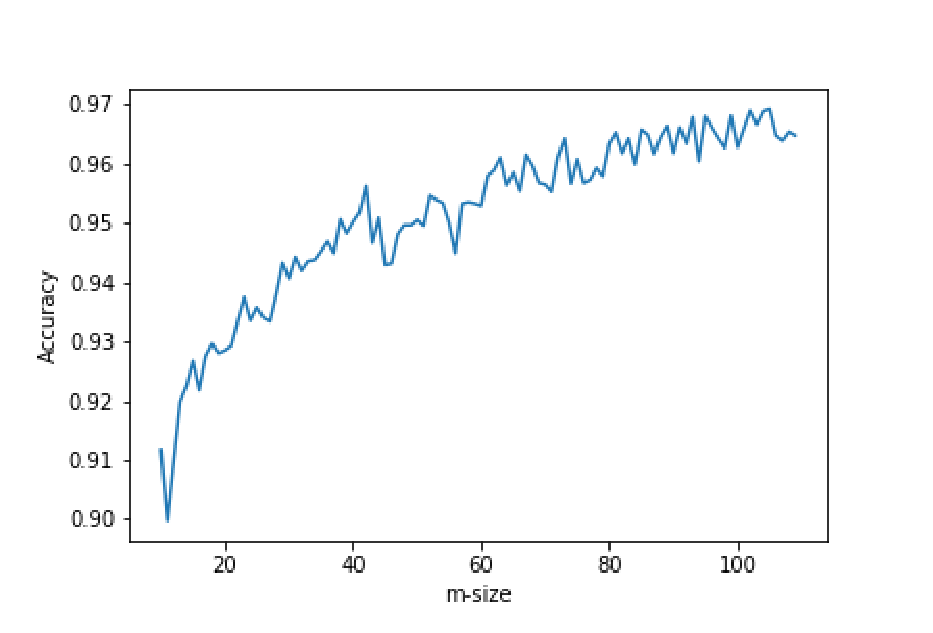
\includegraphics[width=0.5\textwidth]{Accuracy.eps}}
	\subfloat[Функция ошибки log-loss]{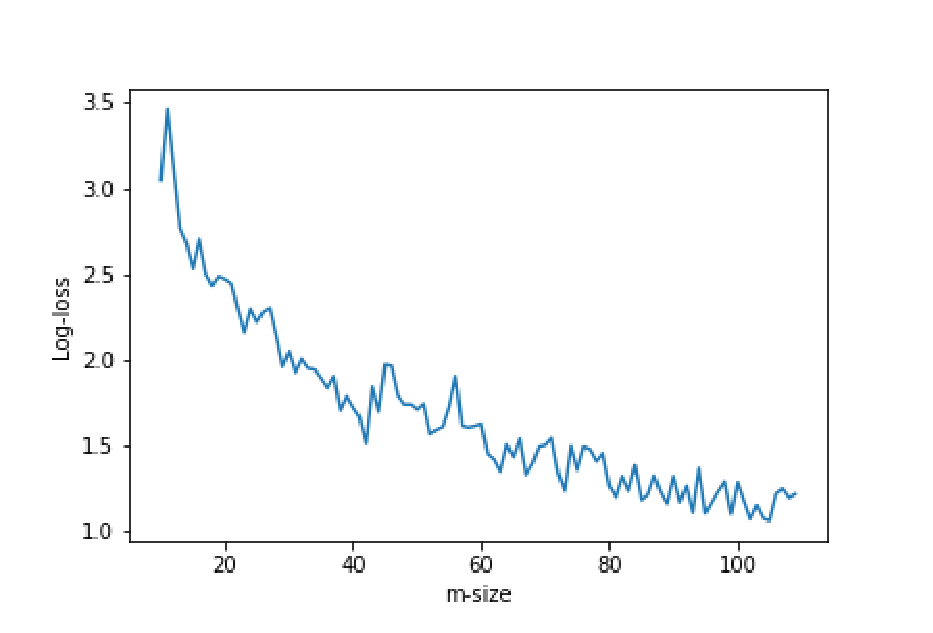
\includegraphics[width=0.5\textwidth]{Log-loss.eps}}\\
	\label{fg:Acc}
\end{figure}

Нетрудно увидеть, что с увеличением объёма выборки качество классификации повышается, однако при добавлении новых данных качество предсказани и ошибки изменяются медленнее. Например, на графике точности количества объектов порядка 20-25 хватает для достижения почти $93\%$ точности. При дальнейшем пополнении выборки, когда объём увеличивается в 5 раз, точность выше только на $3\%$. Ввиду такого факта следует, что не имеет смысла брать выборки очень большого мастштаба для решения реальных задач прогнозирования. В целом, обычно $95\%$ точности является очень хорошим результатом классификации пациентов в медицинской диагностике. Точность выше обычно требуется на data-science соревнованиях, где каждая доля процента крайне важна. Заметим, что в модели логистической регрессии используется стохастический градиентный спук, который чувствителен к параметрам модели. Чтобы процесс нt оказался парализованным и быстрее сходился за определенное число шагов, была произведена нормализация признаков. Из каждого признака вычитается среднее по признаку всех объектов выборки и делится на стандартное отклонение.

Достижение полученных результатов точности на выборках малого объёма появляется не случайно. Этим обоснован выбор модели для нашего эксперимента. Логистическая регрессия очень хорошо работает при выборках небольшого объёма. Другие модели, как например, дерево решений, могут требовать в тысячи раз больше данных. Такой исход можно увидеть в работе \cite{smpltr}. Однако не всегда при помощи простой логистической регрессии удаётся добиться крайне завышенных результатов, как например $95\%$. Для этой цели уже следует использовать усовершенствованные методы классификации. В качестве примера таких методов можно привести многослойный перцептрон.
  

\begin{figure}[h]
	\centering
	\subfloat[Расстояние Кульбака-Лейблера.]{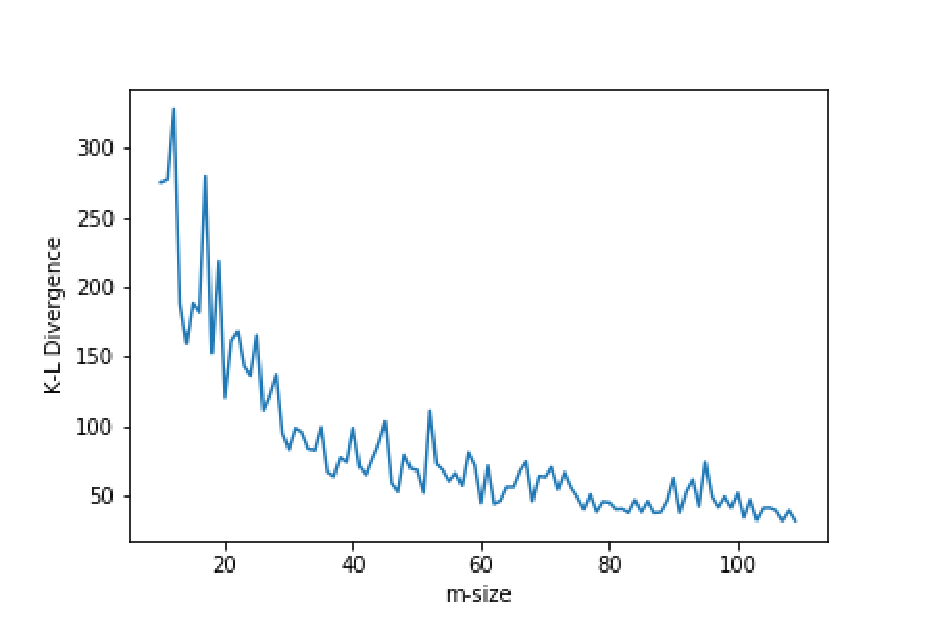
\includegraphics[width=0.5\textwidth]{K-L.eps}}
	\label{fg:kl}
\end{figure}

Стоит внимательно посмотреть на график расстояния Кульбака-Лейблера. Из рисунка можно увидеть, что примерно после объёма ~40 метрика начинает меняться значительно слабее. Таким образом, мы получили оптимальный номер объектов для нашей выборки в модели логистической регрессии.
 

\section{Выводы}
В работе описан алгоритм оценивания оптимального объёма выборки для исследований в медицине. В эксперименте были рассмотрены реальные данные, при помощи которых удалось выявить оптимальное количество элементов для обучения логистической регрессии(приблизительно 40 объектов)

\bibliographystyle{jmlda-rus}
\bibliography{literature}

\end{document}
\grid
